
\subsection{Struktur Aplikasi}
\label{software-structure}

	
	\subsubsection{\textit{Presentation Tier}}
		\textit{Presentation tier} adalah gabungan komponen yang bertanggung jawab terhadap \textit{user interface} ke secara keseluruhan. Dalam \textit{tier} ini  menjadi 2 komponen, yaitu:
		\begin{enumerate}
			\item \textbf{Komponen \textit{View Element}} bertanggungjawab terhadap dari elemen-elemen tampilan (HTML, CSS, JS), juga terkait dengan \textit{templating} (pada penerapannya menggunakan Blade \textit{templating}, yang sudah secara default masuk ke dalam \textit{package} Laravel).
			\item \textbf{Komponen \textit{View Logic}} bertanggungjawab terhadap logika \textit{view}, misal pada halaman melelang barang, maka \textit{view logic} adalah logika program saat pengguna memasukkan penawaran harga, mengklik tombol "Tawar" hingga akhirnya penawaran tersebut sditerima/diproses oleh aplikasi.
		\end{enumerate}
		
		
		\begin{figure}[h]
			\centering
			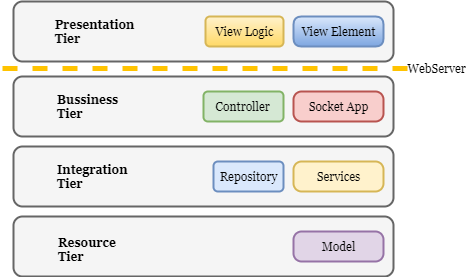
\includegraphics[width=.8\textwidth]{images/bab3/apl/main-apl.png}
			\caption{Komponen Penyusun Struktur Aplikasi}
			\label{software-structure-img}
		\end{figure}
		
	\subsubsection{\textit{Bussiness Tier}}
	\textit{Bussiness tier} adalah gabungan komponen yang bertanggung jawab kelangsungan proses bisnis. Dalam \textit{tier} ini, terdapat 2 komponen yaitu:
	\begin{enumerate}
		\item \textbf{Komponen \textit{Controller}} bertanggungjawab logika/proses bisnis aplikasi secara keseluruhan. \textit{Controller} mengatur autentikasi, otorisasi, penerusan dan pemrosesan \textit{request} dari pengguna kepada komponen pemroses seperti \textit{data management layer} atau \textit{external service layer}, lalu mengembalikan hasilnya kepada pengguna.
		\item \textbf{Komponen \textit{Socket App}}  ditulis dengan menggunakan Node.js, dan komponen ini bertanggungjawab penuh untuk menyediakan \textit{realtime connection} pada fitur berkirim pesan dan proses \textit{bidding}.
	\end{enumerate}
	
	\subsubsection{\textit{Integration Tier}}
	\textit{Integration tier} adalah gabungan komponen yang bertanggung jawab integrasi pemrosesan data dan \textit{external service usages}. Dalam \textit{tier} ini, terdapat komponen-komponen berikut:
	\begin{enumerate}
		\item \textbf{Komponen \textit{Repository}} bertanggungjawab terhadap \textit{data management}, dimana \textit{controller} hanya bertugas meneruskan dan mengautorisasi \textit{request}, maka \textit{repository} bertanggungjawab untuk mengolah data tersebut sesuai permintaan. Lalu, \textit{repository} bertanggungjawab meneruskan status proses (jika sifatnya keberhasilan, misal: \textit{create} data pengguna), atau meneruskan hasil proses (misal: \textit{request} halaman tampilkan barang, maka \textit{repository} bertanggungjawab meneruskan hasil \textit{query} kepada \textit{controller}). \\
		\item \textbf{Komponen \textit{Services}} bertanggungjawab penuh terhadap akses aplikasi ke \textit{external service} seperti SMTP\textit{ Relay} yang menggunakan SendGrid.
	\end{enumerate}

	\subsubsection{\textit{Resource/Data Access Tier}}
	\textit{Resource tier} adalah gabungan komponen yang bertanggungjawab terhadap akses ke \textit{database} dan \textit{storage devices}, yaitu pengaksesan dan \textit{preprocessing} data menjadi \textit{suitable format} bagi komponen lainnya.
	\begin{enumerate}
		\item \textbf{Komponen \textit{Model}} bertanggungjawab terhadap sebuah tabel/entitas dalam \textit{database} aplikasi. Tidak hanya itu, \textit{model} juga bertanggungjawab terhadap \textit{preprocessing} informasi, yaitu pengubahan data dari \textit{database} menjadi \textit{collection}/Eloquent ORM yang merupakan \textit{suitable format} bagi pemrosesan data di tier \textit{repository} maupun \textit{bussiness}.
	\end{enumerate}		
		
	

	
	
	